\chapter{User Interface and Features}
% \label{ch:ui}

\section{Wireframes and User Journey}

Wireframes provide a visual outline of the project's user interface structure and play a key role in mapping the user journey. They enable early visualization of layout and user interactions, offering insight into user navigation within the system well before the detailed design and coding phases.\\
The following wireframes tell the story of a user's journey through the \textbf{ft\_transcendence} platform, from their first interaction to gameplay and beyond.

\subsection{Beginning the Journey: Registration and Authentication}

When first accessing the application, users are presented with the login page. Here, they have two paths to proceed: they can either log in with existing credentials or register a new account.

\begin{figure}[H]
    \centering
    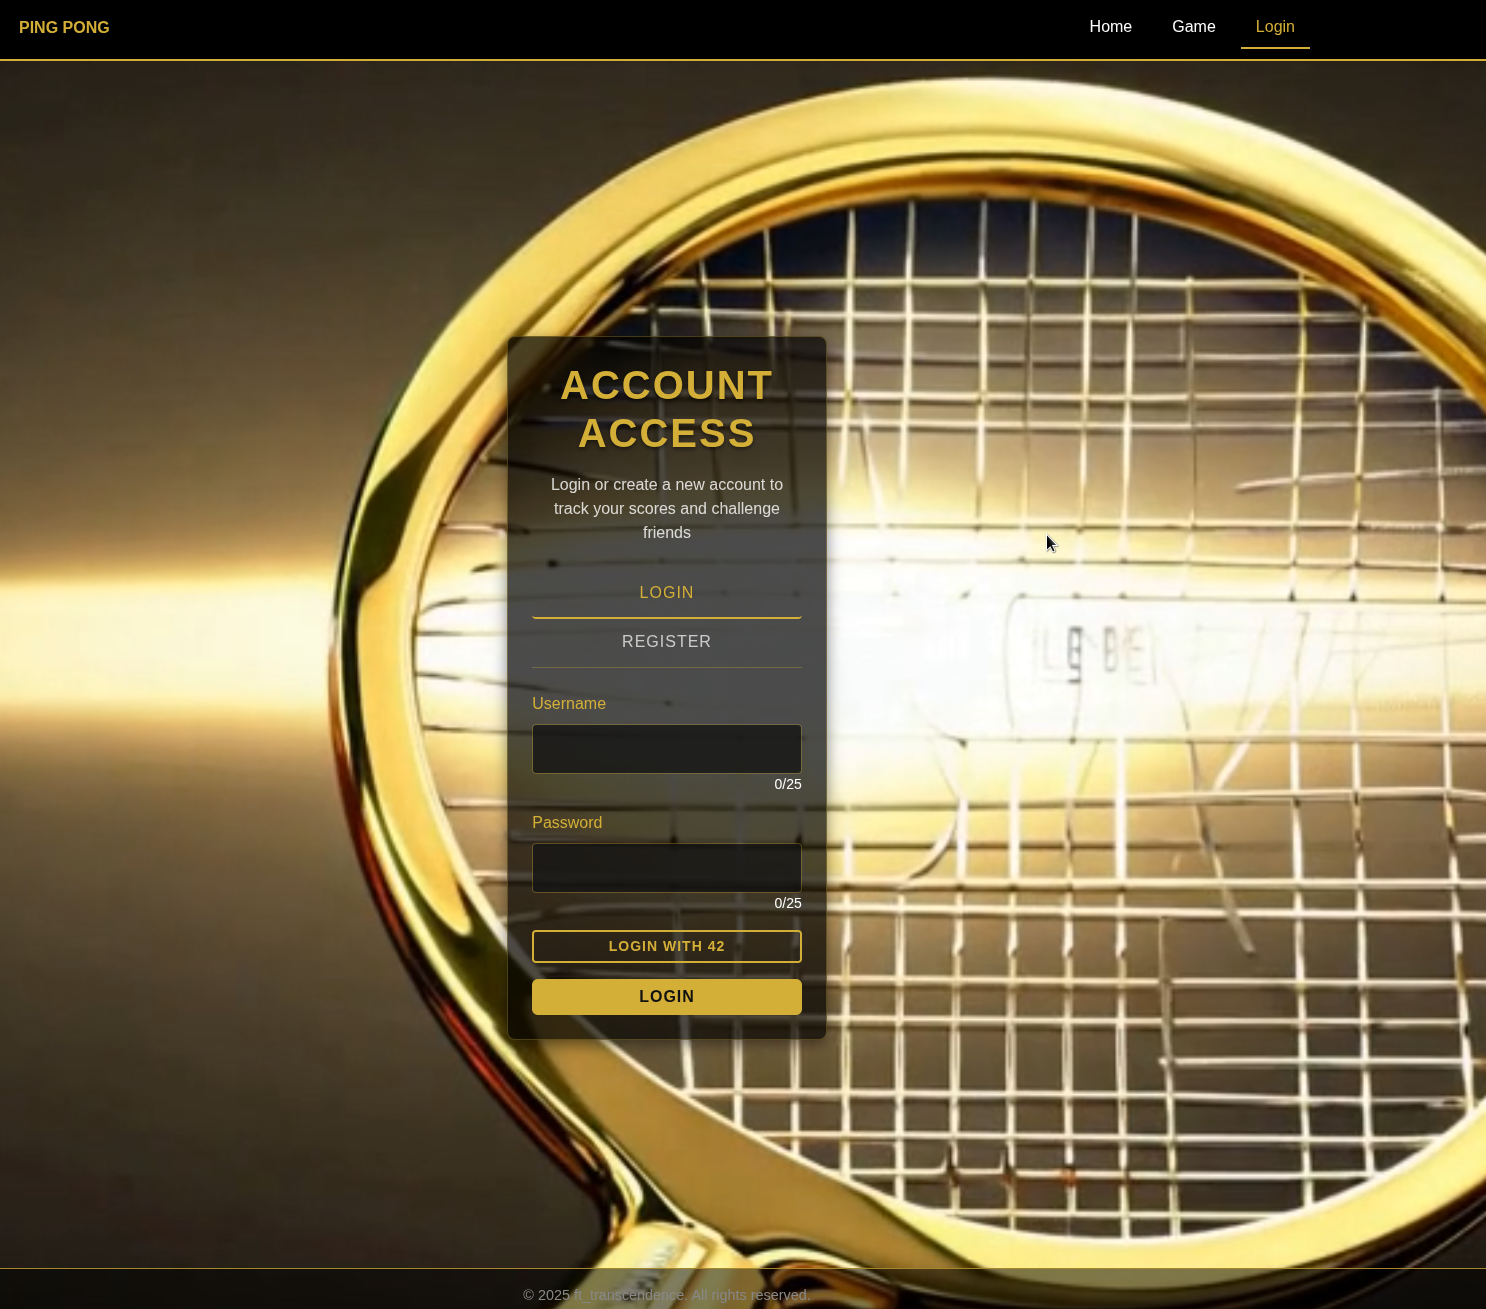
\includegraphics[width=0.7\linewidth]{Figures/images/new_images/LoginPage.png}
    \caption{Login Page.} % Entry point for users with credential-based authentication and 42 OAuth options
    \label{fig:login-page}
\end{figure}

\subsubsection{Path 1: Creating a New Account} For new users, the registration process begins by completing a form with their details. The registration page requires a unique username, valid email address, and secure password.

\begin{figure}[H]
    \centering
    
\includegraphics[width=0.7\linewidth]{Figures/images/new_images/RegistrationPage.png}
    \caption{Registration Page.} % Form for new users to create accounts with validation for username, email and password
    \label{fig:registration-page}
\end{figure}

\begin{figure}[H]
    \centering
    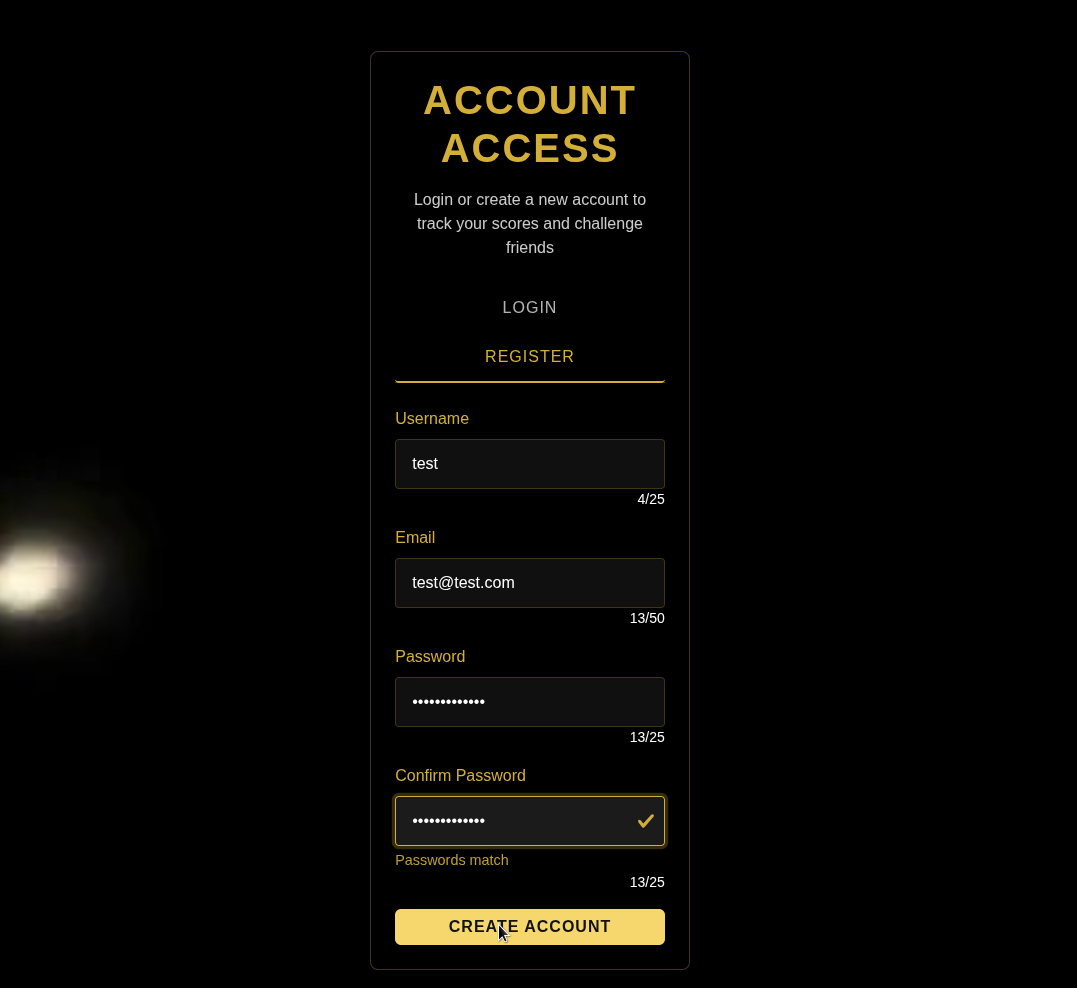
\includegraphics[width=0.7\linewidth]{Figures/images/new_images/RegisteringAccount.png}
    \caption{Account Registration Process.} % Process of filling out registration information
    \label{fig:registering-account}
\end{figure}

During registration, the system validates user input to ensure data quality and security. If a user attempts to submit the form with empty fields, they receive a clear error message:

\begin{figure}[H]
    \centering
    
\includegraphics[width=0.6\linewidth]{Figures/images/new_images/ErrorFillOutAllTheFields.png}
    \caption{Empty Fields Error.} % Validation alert for required form fields
    \label{fig:error-empty-fields-wireframe}
\end{figure}

\begin{figure}[H]
    \centering
    
\includegraphics[width=0.6\linewidth]{Figures/images/new_images/ErrorUserName.png}
    \caption{Username Validation.} % Validation for unique username requirements
    \label{fig:error-username-wireframe}
\end{figure}

The system also validates email format to ensure proper address structure:

\begin{figure}[H]
    \centering
    
\includegraphics[width=0.6\linewidth]{Figures/images/new_images/ErrorEmail.png}
    \caption{Email Validation.} % Email format verification ensuring proper address structure
    \label{fig:error-email-wireframe}
\end{figure}

Passwords must meet security requirements to ensure account protection:

\begin{figure}[H]
    \centering
    
\includegraphics[width=0.6\linewidth]{Figures/images/new_images/ErrorPassword.png}
    \caption{Password Validation.} % Security requirements for creating strong passwords
    \label{fig:error-password-wireframe}
\end{figure}

The system also verifies that password confirmation matches the original entry to prevent typos:

\begin{figure}[H]
    \centering
    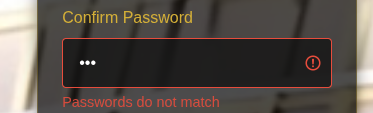
\includegraphics[width=0.6\linewidth]{Figures/images/new_images/ErrorConfirmPassword.png}
    \caption{Password Confirmation.} % Ensuring password entries match during registration
    \label{fig:error-confirm-password-wireframe}
\end{figure}

Upon successful registration, users receive a confirmation message:

\begin{figure}[H]
    \centering
    
\includegraphics[width=0.6\linewidth]{Figures/images/new_images/RegistrationSuccess.png}
    \caption{Registration Success.} % Confirmation of successful account creation
    \label{fig:registration-success-wireframe}
\end{figure}

\subsubsection{Path 2: OAuth with 42 Intra} Alternatively, users with 42 Intra accounts can authenticate through OAuth integration, bypassing the need to create separate credentials:

\begin{figure}[H]
    \centering
    
\includegraphics[width=0.6\linewidth]{Figures/images/new_images/42Login.png}
    \caption{42 Authentication.} % OAuth login option allowing seamless authentication through 42 Intra service
    \label{fig:42-login}
\end{figure}

\begin{figure}[H]
    \centering
    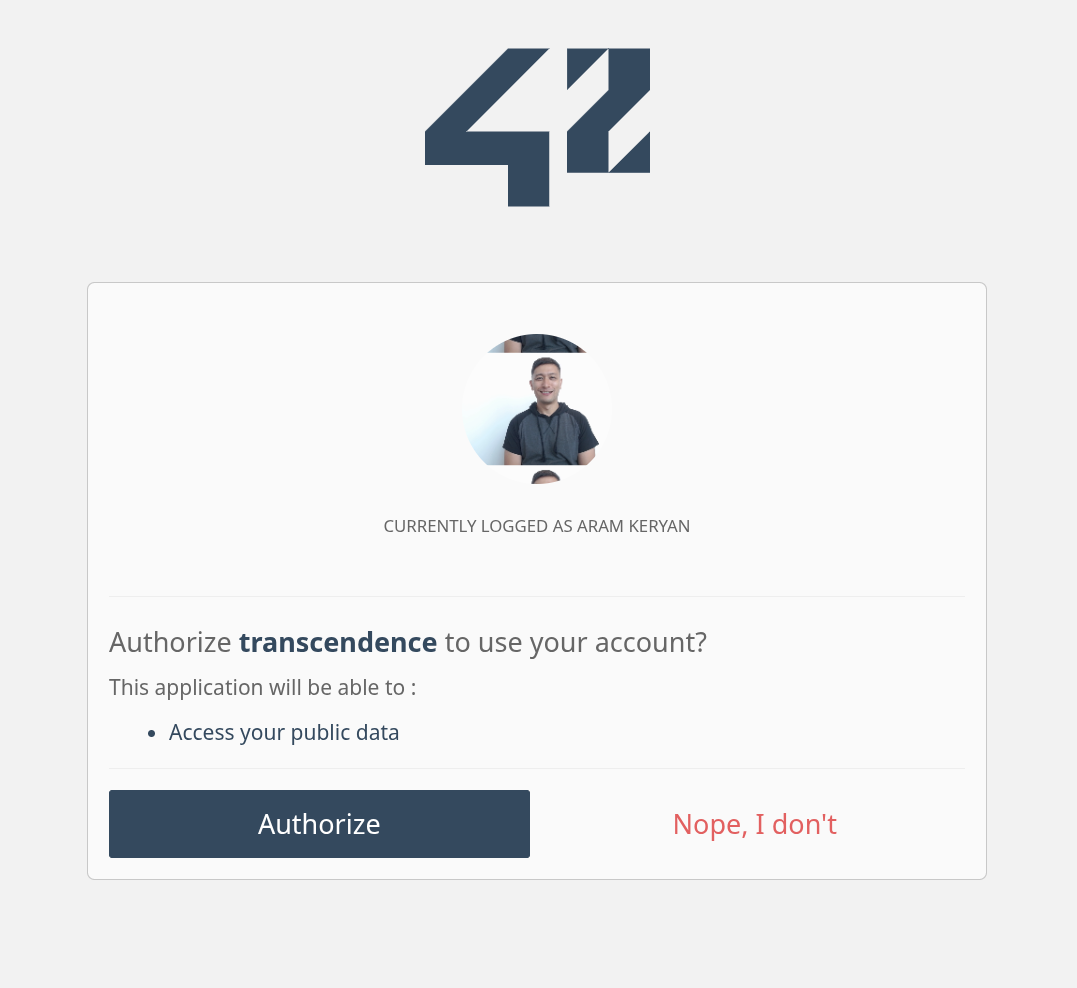
\includegraphics[width=0.6\linewidth]{Figures/images/new_images/42Authentication.png}
    \caption{42 Authentication Process.} % Detailed view of the OAuth authentication process through 42 Intra
    \label{fig:42-auth-process}
\end{figure}

\paragraph{Successful Login} Regardless of the authentication method chosen, upon successful login, users receive a welcome confirmation:

\begin{figure}[H]
    \centering
    
\includegraphics[width=0.6\linewidth]{Figures/images/new_images/LoginSuccessfully.png}
    \caption{Login Success.} % Confirmation of successful authentication
    \label{fig:login-success-wireframe}
\end{figure}

\begin{figure}[H]
    \centering
    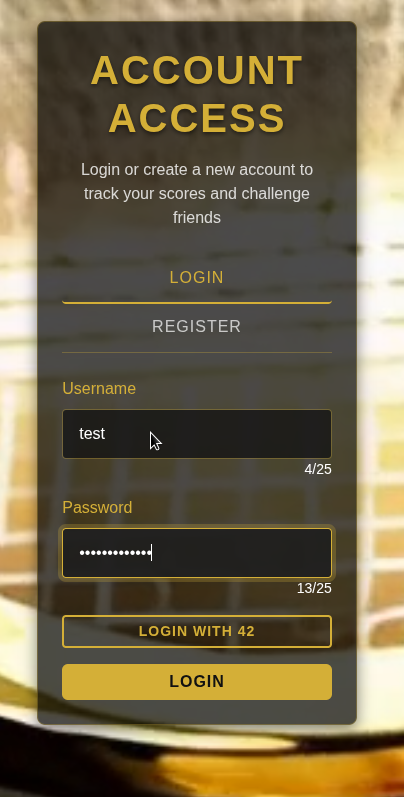
\includegraphics[width=0.6\linewidth]{Figures/images/new_images/LoginWithRegisterdAccount.png}
    \caption{Login With Registered Account.} % Using registered credentials to access the platform
    \label{fig:login-registered-wireframe}
\end{figure}

\subsection{Exploring the Platform: Home Page and Navigation}

After successful login, the user is directed to the home page - the central hub of the application. This modern, clean interface welcomes users and presents the core functionality of the platform.

\begin{figure}[H]
    \centering
    
\includegraphics[width=0.7\linewidth]{Figures/images/new_images/HomePage.png}
    \caption{Home Page.} % Dashboard showing navigation options and available game modes after login
    \label{fig:home-page-journey}
\end{figure}

The application features a consistent navigation menu that appears throughout the platform, ensuring users can always access key sections regardless of where they are in the application. This menu provides quick access to game modes, profile management, friends, and settings.

\begin{figure}[H]
    \centering
    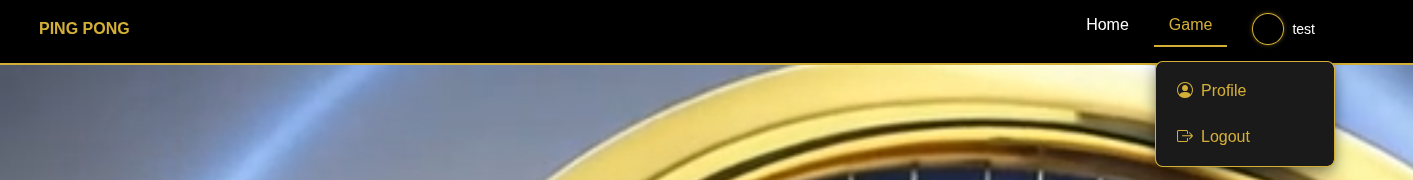
\includegraphics[width=0.65\linewidth]{Figures/images/new_images/MenuBar.png}
    \caption{Menu Bar.} % Navigation providing access to game modes, profile, friends and settings
    \label{fig:menu-bar-journey}
\end{figure}

\subsection{Selecting a Game Mode}

From the home page, users can navigate to the Game page, which serves as the gateway to the core gaming experience. Here, they can select from multiple Pong variants:

\begin{figure}[H]
    \centering
    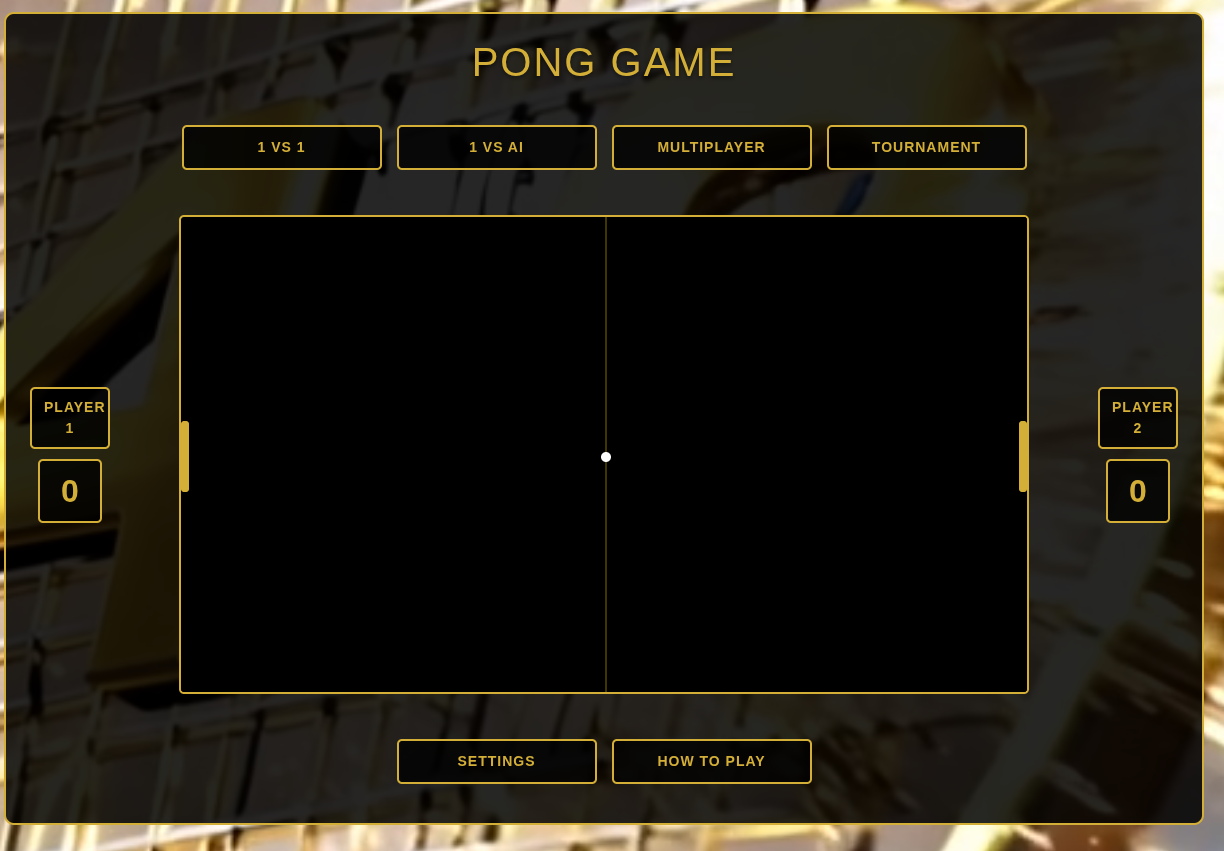
\includegraphics[width=0.7\linewidth]{Figures/images/new_images/GamePage.png}
    \caption{Game Selection.} % Selection hub for different game modes including 1vs1, AI, multiplayer and tournaments
    \label{fig:game-page-journey}
\end{figure}

\subsection{Playing the Game: Exploring Different Game Modes}

Once users have selected a game mode, they enter the actual gameplay experience. The application offers several different ways to enjoy Pong:

\subsubsection{1vs1 Matches} Users can challenge other online players to classic 1vs1 Pong matches. After selecting this mode from the game page, they're taken to the game interface where two human players compete. The screen displays player information, score tracking, and provides intuitive controls (W/S keys for one player, arrow keys for the other).

\begin{figure}[H]
    \centering
    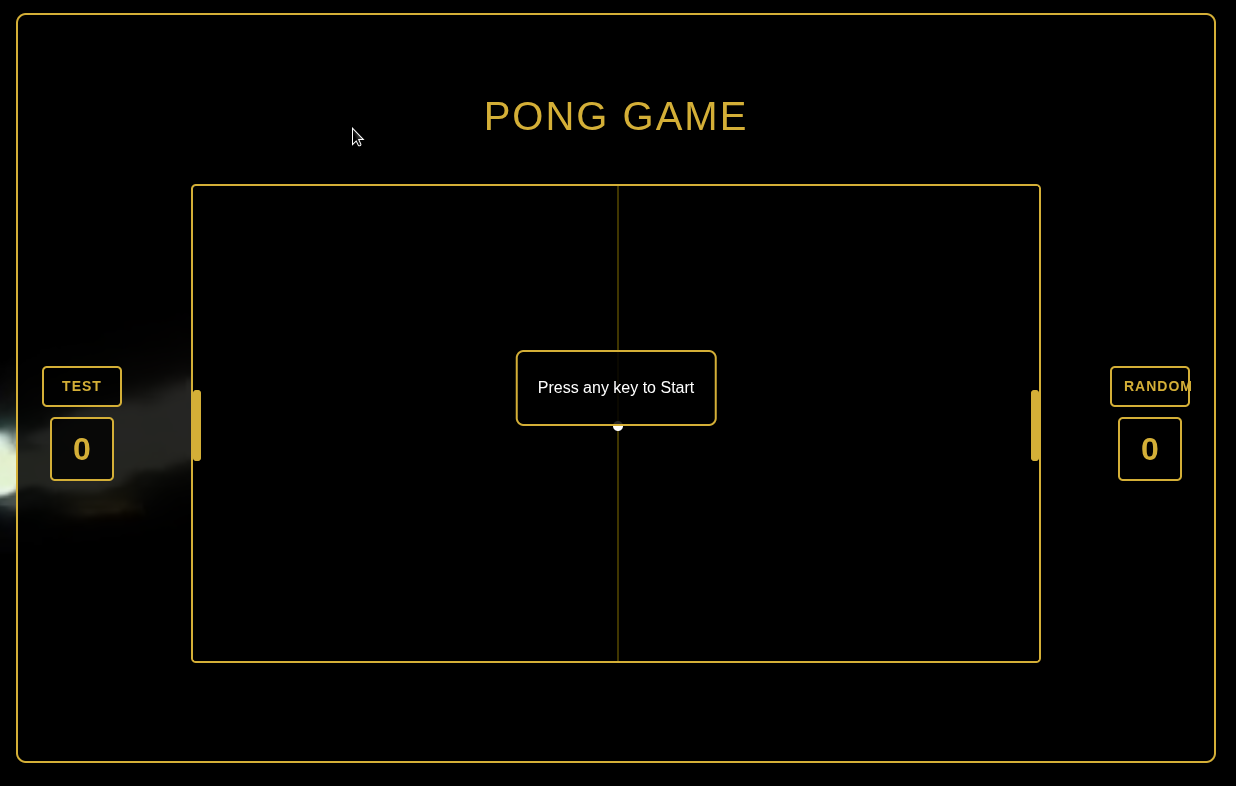
\includegraphics[width=0.65\linewidth]{Figures/images/new_images/Game1vs1.png}
    \caption{1vs1 Game.} % Classic Pong match between two human players with score tracking
    \label{fig:game-1vs1-journey}
\end{figure}

\subsubsection{Practice with AI} For players who want to practice or play solo, the AI opponent mode provides matches against a computer-controlled paddle. This mode maintains the same familiar interface while allowing players to adjust the difficulty level to suit their skill level.

\begin{figure}[H]
    \centering
    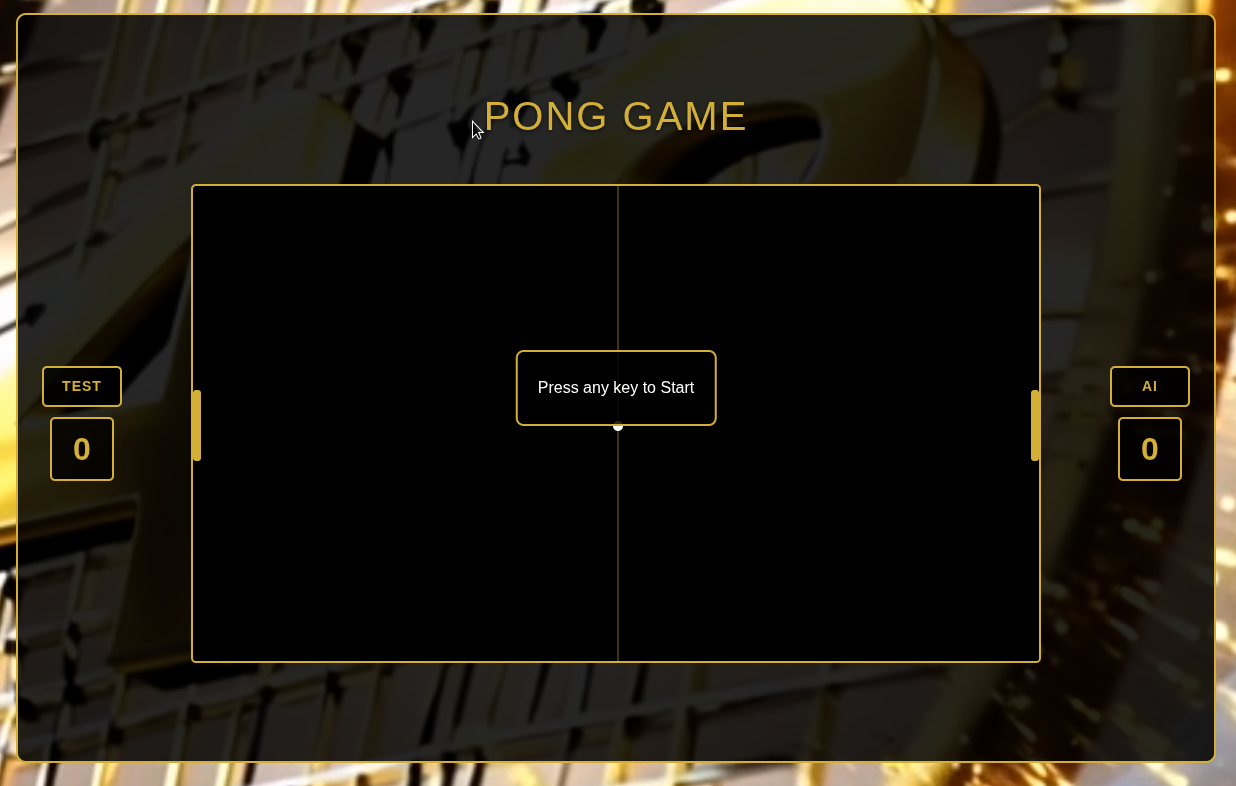
\includegraphics[width=0.65\linewidth]{Figures/images/new_images/Game1vsAI.png}
    \caption{1vs AI Game.} % Practice mode against computer-controlled opponent with adjustable difficulty
    \label{fig:game-1vsai-journey}
\end{figure}

\subsubsection{Local Multiplayer} For social gaming sessions, the multiplayer mode transforms the traditional Pong experience into a dynamic four-player challenge. The interface adapts to place paddles on all four sides of the screen, with each player using different controls for a more social gaming experience.

\begin{figure}[H]
    \centering
    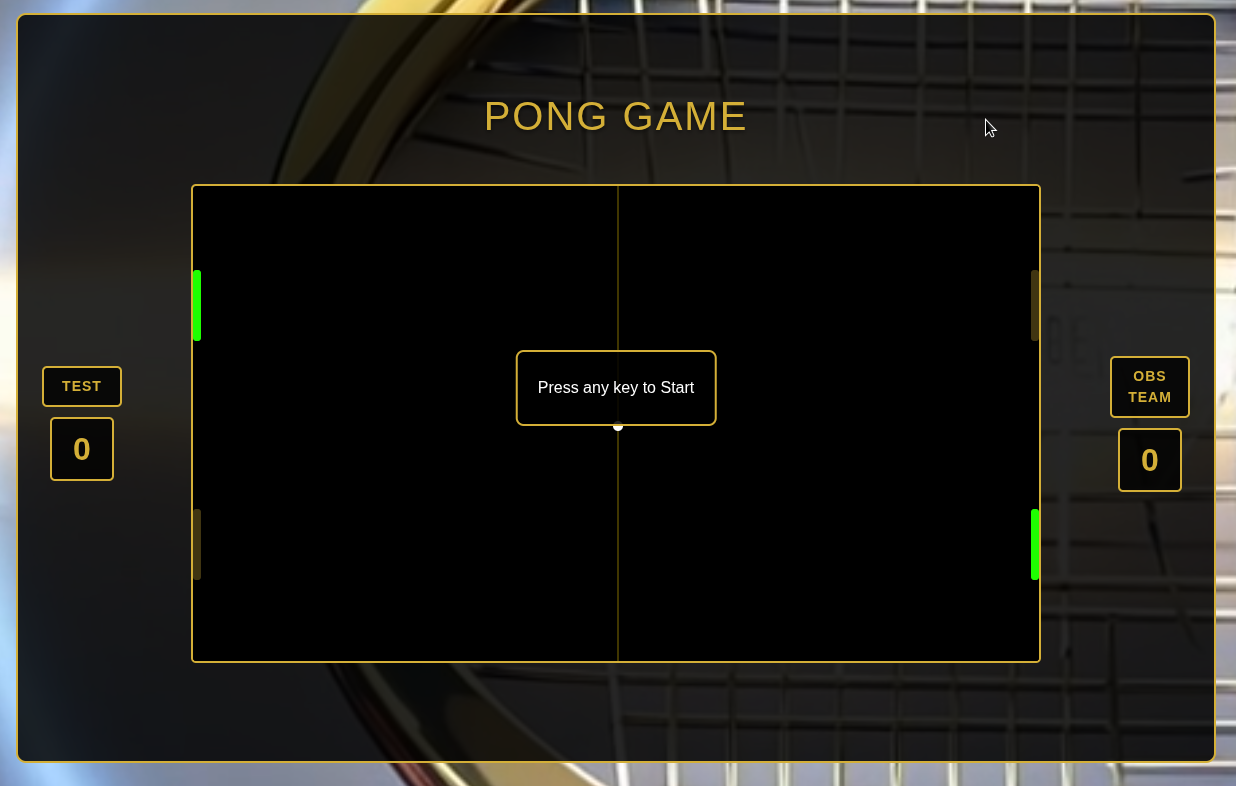
\includegraphics[width=0.65\linewidth]{Figures/images/new_images/GameMultiPlayer.png}
    \caption{Multiplayer Mode.} % Four-player variation with paddles on all sides for local gameplay
    \label{fig:multiplayer-game-journey}
\end{figure}

\subsubsection{Customizing the Experience} Players can personalize their gaming experience through the settings interface. Here they can adjust various parameters including visual preferences, sound options, control layouts, and AI difficulty levels.

\begin{figure}[H]
    \centering
    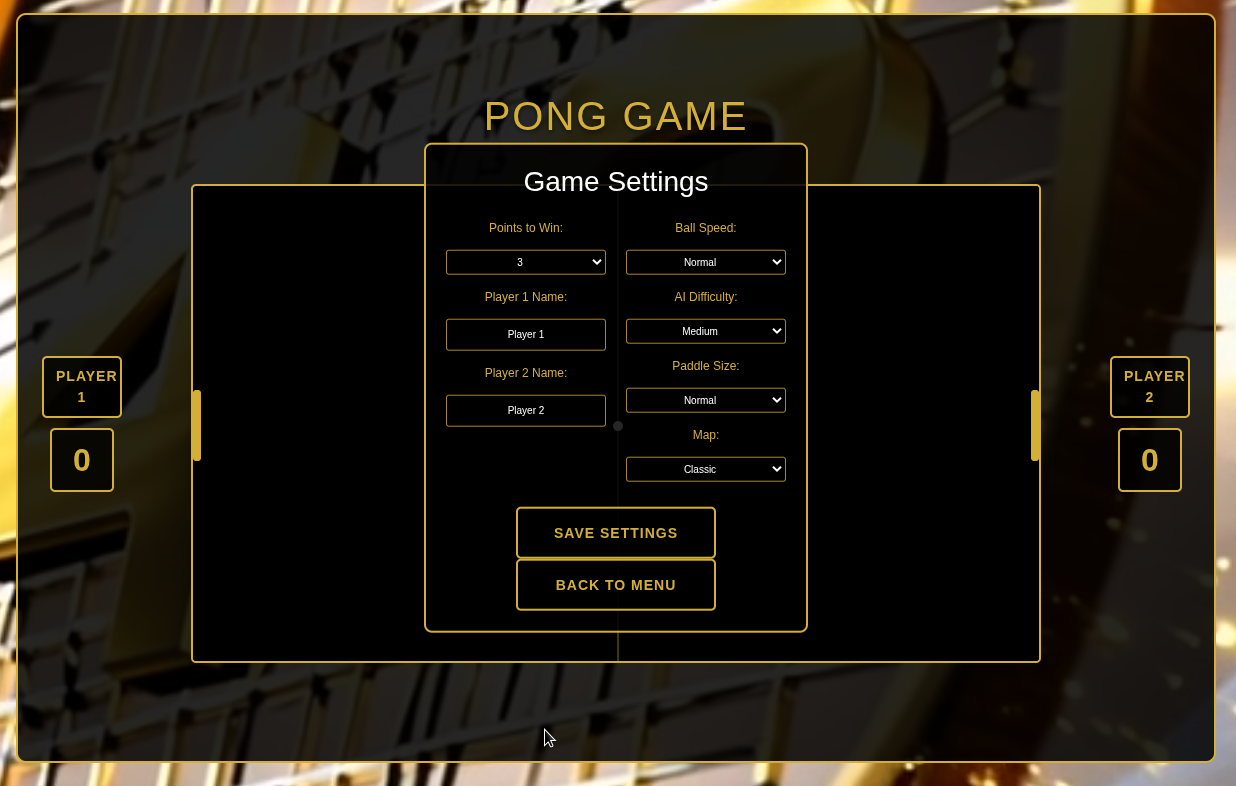
\includegraphics[width=0.65\linewidth]{Figures/images/new_images/GameSettings.png}
    \caption{Game Settings.} % Configuration options for customizing gameplay parameters and preferences
    \label{fig:game-settings-journey}
\end{figure}

\subsubsection{End of Match} When a game concludes, the results screen displays the outcome, final score, and performance statistics. From here, players can choose to play again or return to the main menu.

\begin{figure}[H]
    \centering
    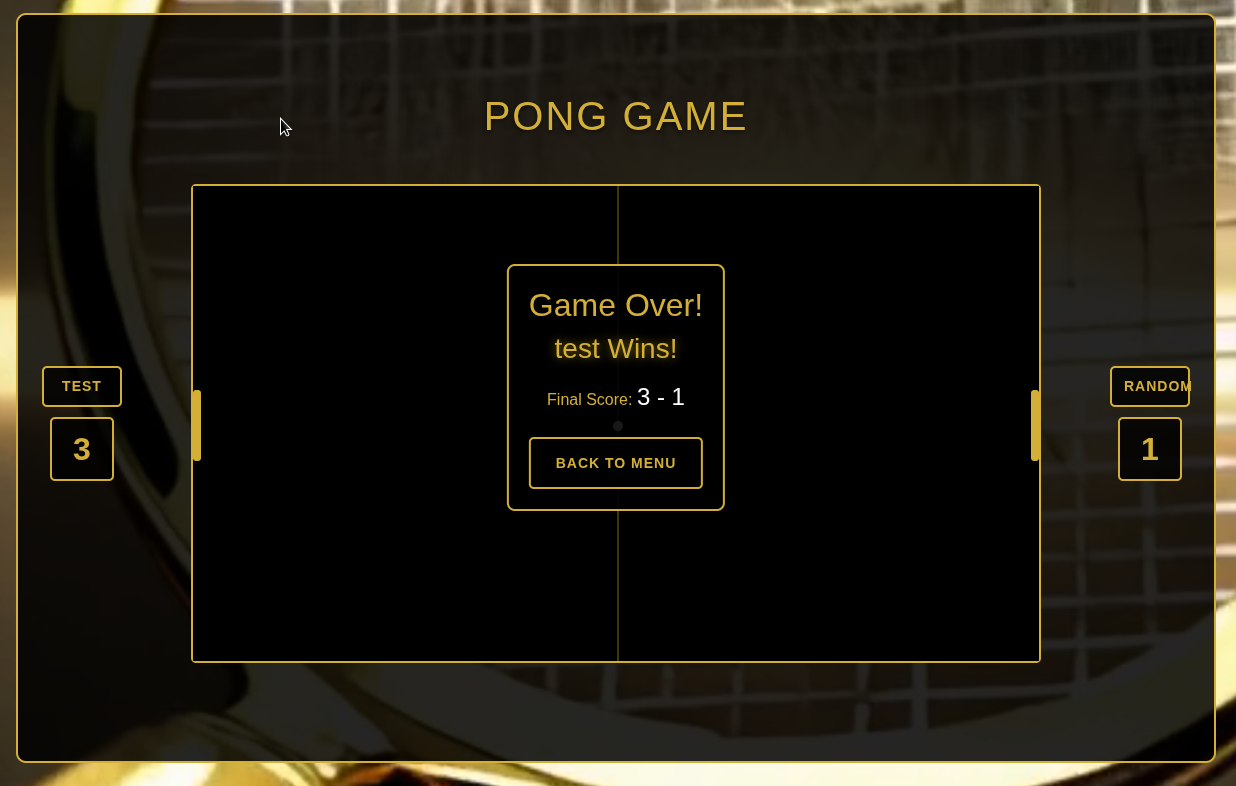
\includegraphics[width=0.65\linewidth]{Figures/images/new_images/GameResult.png}
    \caption{Game Results.} % Match outcome showing final score and player performance statistics
    \label{fig:game-result-journey}
\end{figure}

\subsection{Competing in Tournaments}

For users seeking more structured competition, the tournament mode offers an organized bracket-style experience. After selecting this option from the game page, the user journey continues with tournament participation.

\subsubsection{Joining a Tournament} Users first see the tournament bracket interface that displays all participants and the structure of the competition. Here they can view their position in the bracket, upcoming matches, and track the overall progress of the tournament.

\begin{figure}[H]
    \centering
    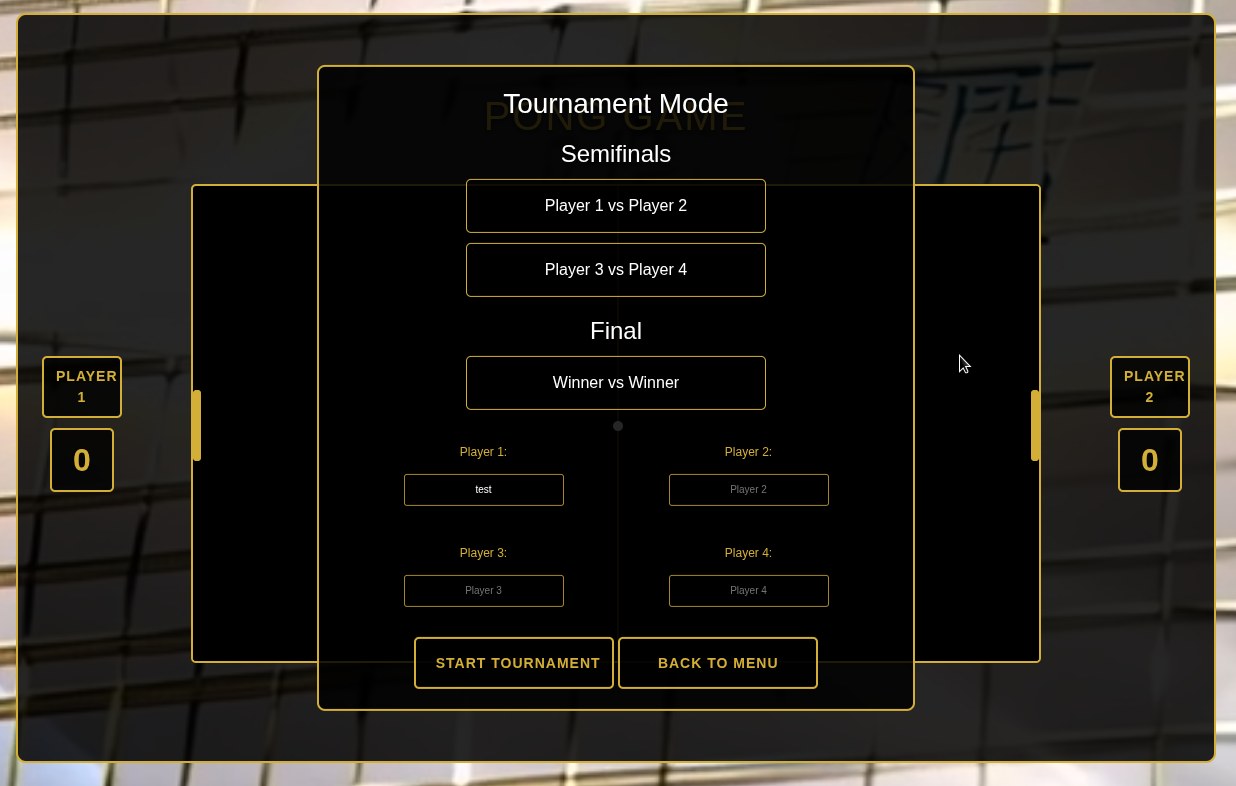
\includegraphics[width=0.65\linewidth]{Figures/images/new_images/GameTournament.png}
    \caption{Tournament Bracket.} % Structured competition showing participating players and bracket progression
    \label{fig:tournament-bracket-journey}
\end{figure}

\subsubsection{Advancing Through Rounds} As users win matches, they progress through the tournament bracket. The semi-final matches maintain the same core gameplay mechanics while highlighting the heightened stakes of the elimination round.

\begin{figure}[H]
    \centering
    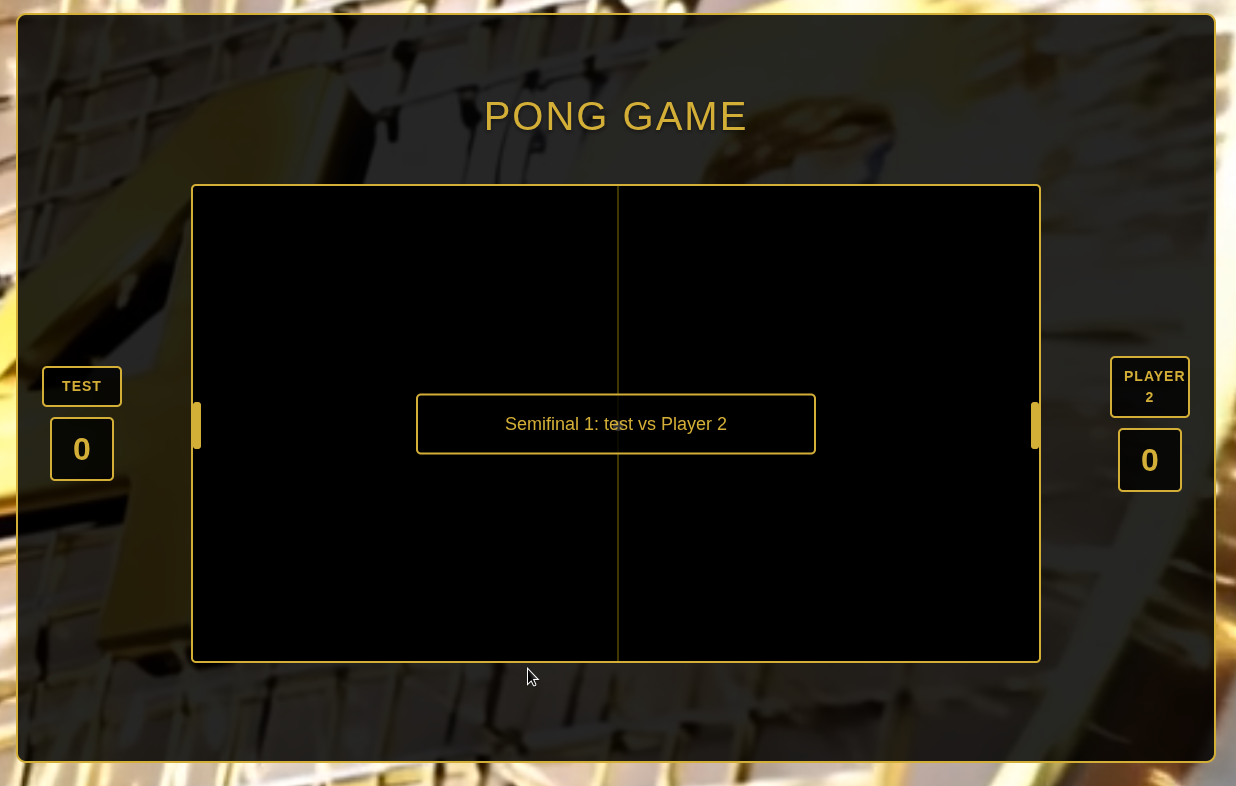
\includegraphics[width=0.65\linewidth]{Figures/images/new_images/GameTournementSemiFinal1.png}
    \caption{Semi-Final Match.} % Tournament elimination round between qualifying players
    \label{fig:tournament-semifinal-journey}
\end{figure}

\subsubsection{Championship} The tournament journey culminates in the final match between the two remaining players. The stakes are highest here, as results from championship matches are not only recorded in the PostgreSQL database but also immutably stored on the Ethereum sidechain, providing a permanent record of achievement.

\begin{figure}[H]
    \centering
    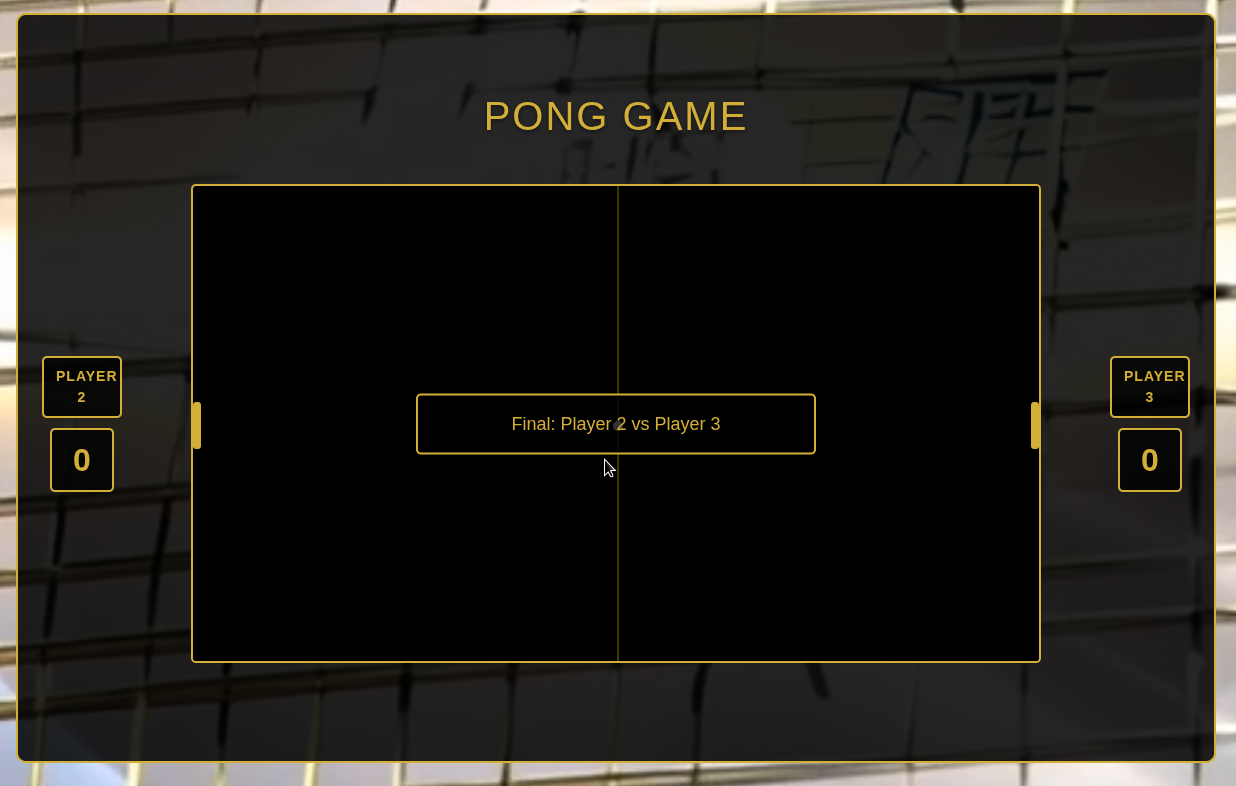
\includegraphics[width=0.65\linewidth]{Figures/images/new_images/GameTournementFinal.png}
    \caption{Tournament Final.} % Championship match with results recorded in database and blockchain
    \label{fig:tournament-final-journey}
\end{figure}

\subsection{Managing Your Profile and Tracking Progress}

Between gaming sessions, users will likely want to review their performance and manage their profile information. The application provides comprehensive profile management tools accessible from the main navigation bar.

\subsubsection{Viewing Your Profile} Users can access their profile page to view their personal statistics, including win/loss ratios, average scores, and ranking information. The profile interface serves as both a personal dashboard and a public-facing representation when viewed by other users.

\begin{figure}[H]
    \centering
    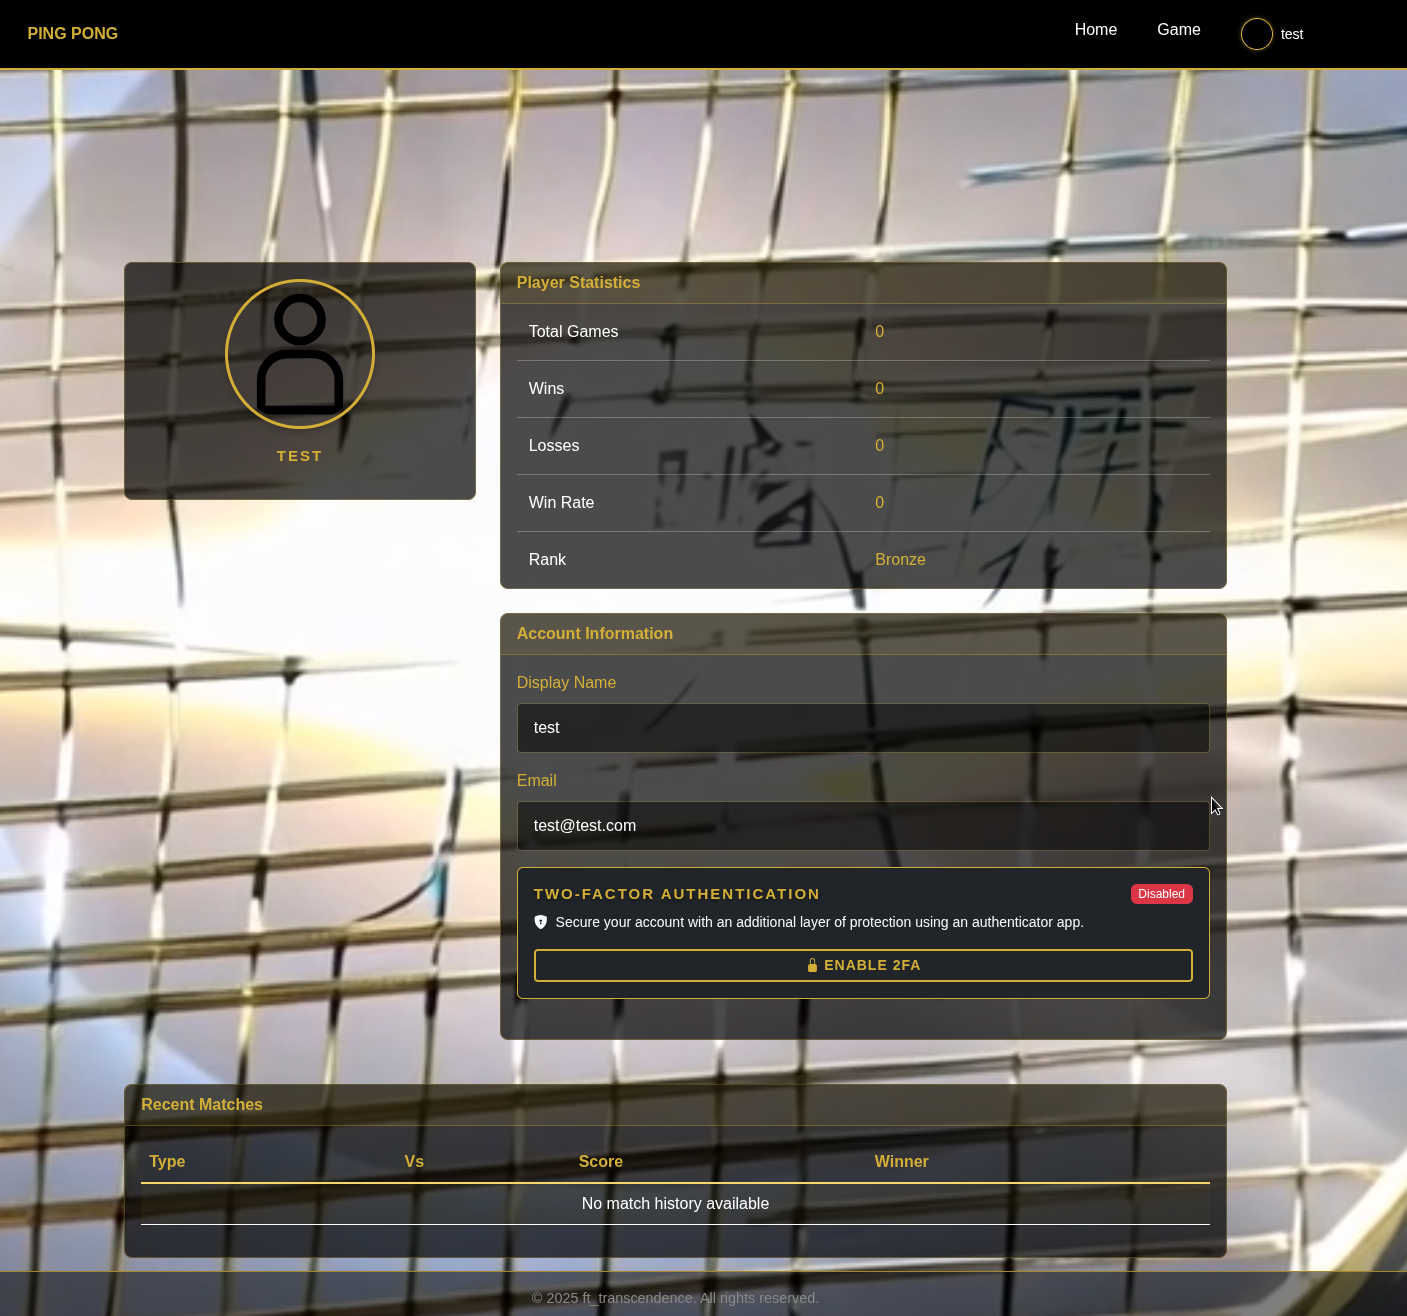
\includegraphics[width=0.65\linewidth]{Figures/images/new_images/ProfilePage.png}
    \caption{User Profile.} % Personal dashboard showing user information and statistics
    \label{fig:profile-page-journey}
\end{figure}

\subsubsection{Reviewing Game History} To help users track their progress and improvement over time, the match history section provides a chronological record of past games. Here users can see their opponents, game outcomes, and performance metrics from previous matches.

\begin{figure}[H]
    \centering
    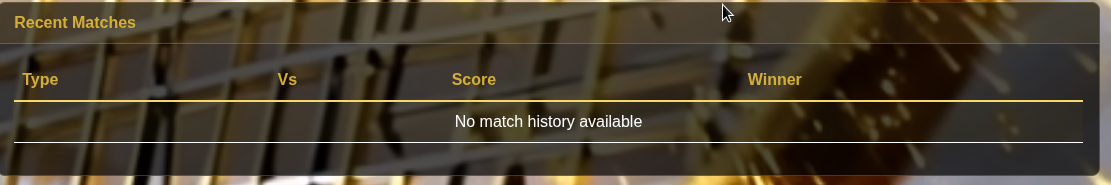
\includegraphics[width=0.65\linewidth]{Figures/images/new_images/History.png}
    \caption{Match History.} % Chronological list of past games with outcomes and statistics
    \label{fig:match-history-journey}
\end{figure}

\begin{figure}[H]
    \centering
    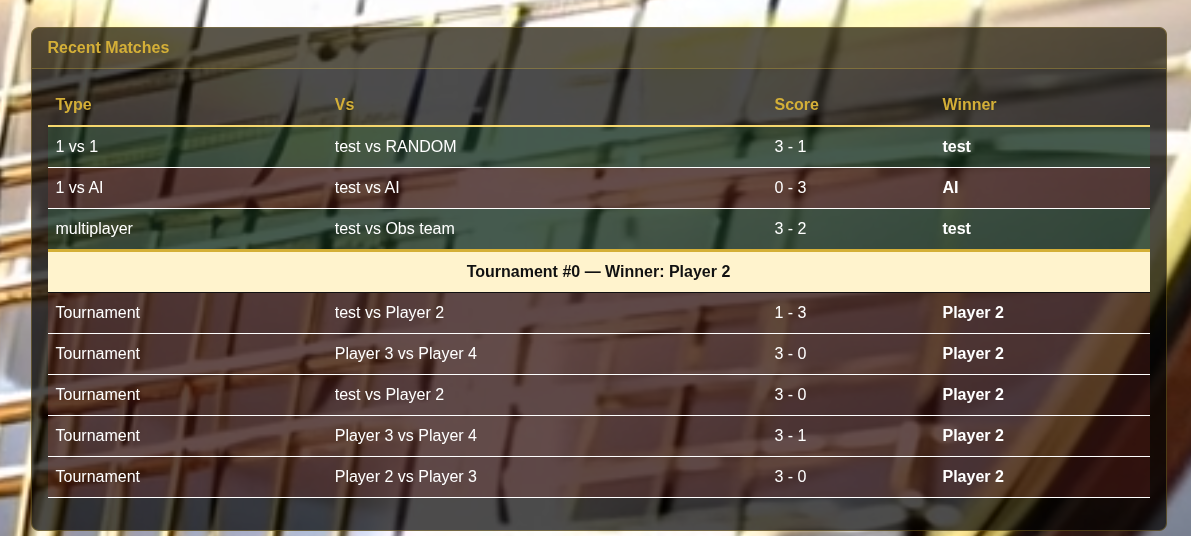
\includegraphics[width=0.65\linewidth]{Figures/images/new_images/RecentMatchesWithData.png}
    \caption{Recent Matches with Data.} % Detailed view of recent match data and statistics
    \label{fig:recent-matches-data-journey}
\end{figure}

\subsubsection{Tracking Performance} Beyond basic profile information, users can access detailed statistics about their gameplay performance. This includes wins and losses, points scored, average game duration, and other performance metrics that help track improvement over time.

\begin{figure}[H]
    \centering
    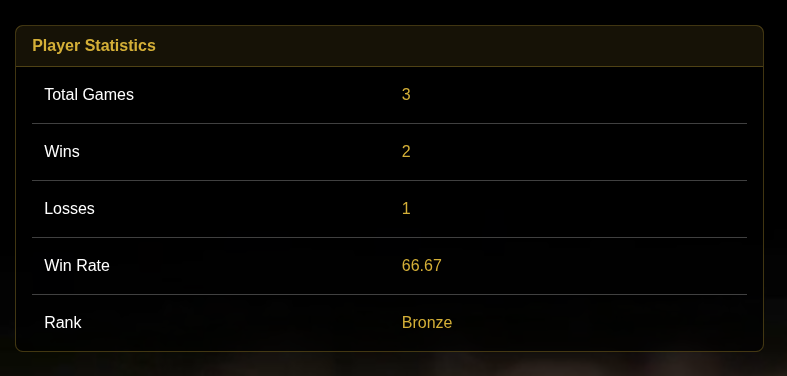
\includegraphics[width=0.65\linewidth]{Figures/images/new_images/PlayerStatisticsWithData.png}
    \caption{Player Statistics.} % Detailed performance metrics and gameplay history
    \label{fig:player-stats-journey}
\end{figure}

\subsection{Managing Your Account and Security}

As users become more engaged with the platform, they may want to personalize their experience further and enhance their account security. The application provides comprehensive account management tools accessible from the navigation menu.

\subsubsection{Account Information} The account settings page displays the user's account details and information. Users can view their account information in this section.

\begin{figure}[H]
    \centering
    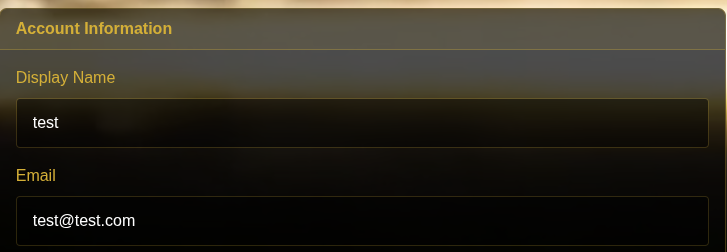
\includegraphics[width=0.65\linewidth]{Figures/images/new_images/AccountInformation.png} % Settings.png not available, using EditProfile as substitute
    \caption{Account Information.} % Page displaying account details
    \label{fig:settings-journey}
\end{figure}

\subsubsection{Enhancing Security} As part of best security practices, the platform offers two-factor authentication (2FA). Users who want to protect their accounts can enable this feature through a guided setup process, linking an authentication app to provide an additional layer of security beyond just a password.

\begin{figure}[H]
    \centering
    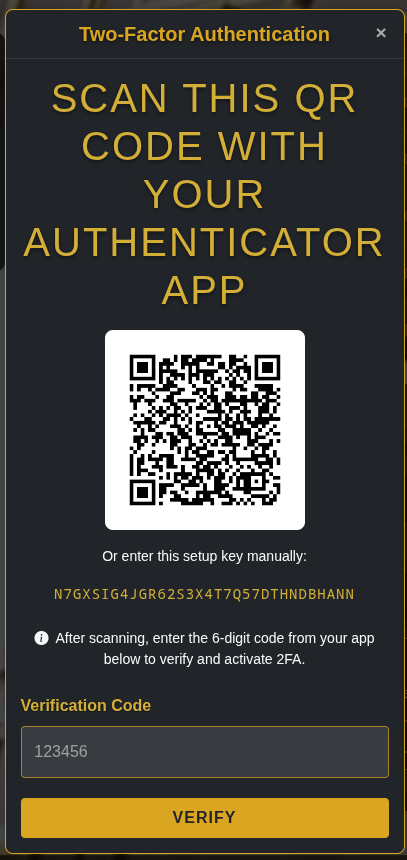
\includegraphics[width=0.4\linewidth]{Figures/images/new_images/Enabling2FA.png}
    \caption{Two-Factor Setup.} % Interface for enabling two-factor authentication security
    \label{fig:2fa-setup-journey}
\end{figure}

\subsubsection{Security Confirmation} After completing the 2FA setup, users receive confirmation that their additional security layer is active. The confirmation screen also provides recovery options to ensure they can regain access if their authentication device is lost or unavailable.

\begin{figure}[H]
    \centering
    
\includegraphics[width=0.65\linewidth]{Figures/images/new_images/2FASuccessfullyEnabled.png}
    \caption{Security Confirmation.} % Successful setup of two-factor authentication
    \label{fig:2fa-confirmation-journey}
\end{figure}

\subsubsection{Two-Factor Authentication Status} Users can verify the status of their two-factor authentication. The platform clearly indicates whether 2FA is currently enabled or disabled for their account.

\begin{figure}[H]
    \centering
    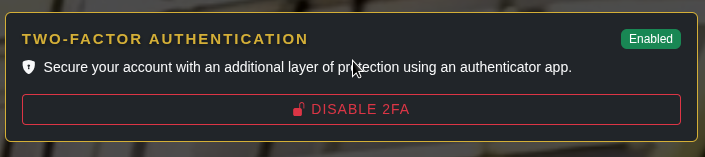
\includegraphics[width=0.65\linewidth]{Figures/images/new_images/2FAEnabled.png}
    \caption{2FA Enabled Status.} % Visual indication that two-factor authentication is active
    \label{fig:2fa-enabled-journey}
\end{figure}

\begin{figure}[H]
    \centering
    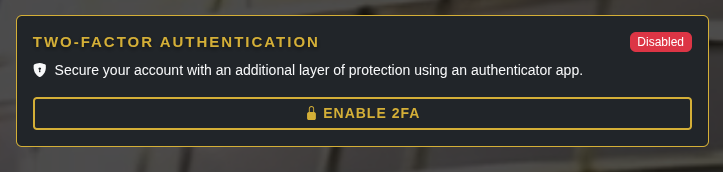
\includegraphics[width=0.65\linewidth]{Figures/images/new_images/2FADisabled.png}
    \caption{2FA Disabled Status.} % Visual indication that two-factor authentication is inactive
    \label{fig:2fa-disabled-journey}
\end{figure}

\subsection{Ending Your Session: Logout}

When users are ready to end their session, the application provides a straightforward logout process.

\subsubsection{Logout Process} Users can access the logout option from the navigation menu. Upon selecting logout, the system securely terminates their session and displays a confirmation message.

\begin{figure}[H]
    \centering
    
\includegraphics[width=0.65\linewidth]{Figures/images/new_images/LogoutSuccessfully.png}
    \caption{Logout Confirmation.} % Notification of successful session termination
    \label{fig:logout-confirmation-journey}
\end{figure}

\subsubsection{Journey Completion} After logout, users are redirected to the login page, completing the full user journey cycle. This clear boundary between sessions helps maintain security while providing an obvious re-entry point for the next visit.

\subsection{Form Validation Throughout the Journey}

Throughout the user journey, the application implements comprehensive form validation to ensure data integrity and provide clear feedback:

\subsubsection{Empty Field Validation} When forms are submitted with missing information, the system displays targeted validation messages.

\begin{figure}[H]
    \centering
    
\includegraphics[width=0.65\linewidth]{Figures/images/new_images/ErrorFillOutAllTheFields.png}
    \caption{Empty Fields Alert.} % Validation message for incomplete form submission
    \label{fig:error-empty-fields-journey}
\end{figure}

\subsubsection{Email Format Validation} The system verifies that email addresses conform to proper formatting standards.

\begin{figure}[H]
    \centering
    
\includegraphics[width=0.65\linewidth]{Figures/images/new_images/ErrorEmail.png}
    \caption{Email Format Alert.} % Validation message for incorrectly formatted email address
    \label{fig:error-email-journey}
\end{figure}

\subsubsection{Password Requirements} To enhance security, the application enforces password strength policies.

\begin{figure}[H]
    \centering
    
\includegraphics[width=0.65\linewidth]{Figures/images/new_images/ErrorPassword.png}
    \caption{Password Strength Alert.} % Validation message for password that doesn't meet security requirements
    \label{fig:error-password-journey}
\end{figure}

\subsubsection{Password Matching} The system ensures that password confirmation fields match the initially entered password.

\begin{figure}[H]
    \centering
    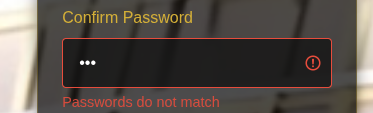
\includegraphics[width=0.65\linewidth]{Figures/images/new_images/ErrorConfirmPassword.png}
    \caption{Password Mismatch Alert.} % Error message when password and confirmation don't match
    \label{fig:error-confirm-password-journey}
\end{figure}

\subsection{Journey Conclusion}

The wireframes presented in this chapter illustrate the complete user journey through the ft\_transcendence application, from initial registration to gameplay and eventual logout. This cohesive flow demonstrates how the various screens and interfaces work together to create a seamless user experience that is both intuitive and engaging.

The journey begins with authentication, progresses through exploration of the platform's features and gameplay, allows for social interaction and profile management, provides security options, and concludes with a clear session ending. Throughout this journey, users encounter consistent navigation patterns, clear feedback mechanisms, and intuitive interfaces that collectively deliver a polished and professional gaming experience.
